\documentclass[a4paper,12pt]{article}
\usepackage[utf8]{inputenc}
\usepackage[german]{babel}
\usepackage{amsmath}
\usepackage{amssymb}
\usepackage{amsthm}
\usepackage{geometry}
\usepackage{graphicx}
\usepackage[hidelinks]{hyperref}
\usepackage{listings}
\usepackage{xcolor}
\usepackage{algorithm}
\usepackage{algpseudocode}
\usepackage{chngcntr}

\geometry{margin=2.5cm}

\theoremstyle{definition}
\newtheorem{definition}{Definition}
\newtheorem{beispiel}{Beispiel}
\newtheorem{satz}{Satz}
\newtheorem{lemma}{Lemma}
\newtheorem{korollar}{Korollar}
\counterwithin{algorithm}{section}

% Code-Highlighting
\lstset{
	basicstyle=\ttfamily\small,
	keywordstyle=\color{blue},
	commentstyle=\color{gray},
	stringstyle=\color{red},
	numbers=left,
	numberstyle=\tiny,
	breaklines=true,
	frame=single
}

\title{Boolean Matrixmultiplikation in $O(n^2)$ \\
\large Anwendung des Signatur-Verfahrens aus dem Subgraph Algorithmus}
\author{Stephan Epp}
\date{\today}

\begin{document}
	
\maketitle

\begin{abstract}
	Dieses Dokument beschreibt eine Anwendung der Signatur-Technik aus dem Subgraph Algorithmus auf die Boolean Matrixmultiplikation. Während die allgemeine Matrixmultiplikation eine Komplexität von mindestens $\Omega(n^{2.37})$ hat, wird gezeigt, dass Boolean Matrixmultiplikation mit der Signatur-Methode in $O(n^2)$ Zeit berechnet werden kann. Dies wird durch geschickte Nutzung von Bitoperationen und polynomialer Hash-Kodierung erreicht.
\end{abstract}

\tableofcontents
\newpage

\section{Einführung}

Die klassische Matrixmultiplikation zweier $n \times n$ Matrizen $A$ und $B$ berechnet eine Ergebnismatrix $C$ mit:
\begin{align}
C_{ij} = \sum_{k=1}^{n} A_{ik} \cdot B_{kj}
\end{align}
Die naive Implementierung hat eine Laufzeit von $O(n^3)$. Fortgeschrittene Algorithmen wie \textsc{Strassen} (1969) oder \textsc{Coppersmith-Winograd} (1990) erreichen $O(n^{2.807})$ bzw. $O(n^{2.376})$.

Für \textbf{Boolean Matrizen}, bei denen alle Einträge $\{0, 1\}$ sind und die Operationen durch logische Operationen ersetzt werden, kann die Signatur-Technik aus dem Subgraph Algorithmus genutzt werden, um eine Laufzeit von $O(n^2)$ zu erreichen.

\begin{definition}[Boolean Matrixmultiplikation]
	Für zwei Boolean Matrizen $A, B \in \{0,1\}^{n \times n}$ ist die Boolean Matrixmultiplikation definiert als:
	\[
	C_{ij} = \bigvee_{k=1}^{n} (A_{ik} \wedge B_{kj})
	\]
	wobei $\vee$ das logische ODER und $\wedge$ das logische UND bezeichnet.
\end{definition}

Mit anderen Worten: $C_{ij} = 1$ genau dann, wenn es mindestens ein $k$ gibt mit $A_{ik} = 1$ und $B_{kj} = 1$.

Die zentrale Idee aus dem Subgraph Algorithmus ist die Verwendung einer polynomialen Hash-Funktion zur Kodierung von Binärvektoren:

\begin{definition}[Signatur-Funktion]
	Für einen Binärvektor $v = (v_0, v_1, \ldots, v_{n-1}) \in \{0,1\}^n$ ist die Signatur definiert als:
	\begin{align}
	\sigma(v) = \sum_{i=0}^{n-1} v_i \cdot 2^i
	\end{align}
\end{definition}

\begin{beispiel}
	Für $v = (1, 0, 1, 1)$ ergibt sich:
	\[
	\sigma(v) = 1 \cdot 2^0 + 0 \cdot 2^1 + 1 \cdot 2^2 + 1 \cdot 2^3 = 1 + 4 + 8 = 13
	\]
\end{beispiel}

\begin{lemma}[Eindeutigkeit]
	Die Signatur-Funktion $\sigma: \{0,1\}^n \to \mathbb{N}$ ist injektiv.
\end{lemma}

\begin{proof}
	Die Signatur entspricht der Interpretation des Binärvektors als Dezimalzahl in Binärdarstellung. Verschiedene Binärvektoren ergeben verschiedene Dezimalzahlen im Bereich $[0, 2^n-1]$.
\end{proof}

Die Signatur hat eine wichtige algebraische Eigenschaft bezüglich der bitweisen UND-Operation:

\begin{lemma}[Bitweise UND-Operation]
	Seien $v, w \in \{0,1\}^n$ zwei Binärvektoren mit Signaturen $\sigma(v)$ und $\sigma(w)$. Dann gilt:
	\[
	\sigma(v) \; \& \; \sigma(w) = \sigma(v \wedge w)
	\]
	wobei $\&$ die bitweise UND-Operation auf den Dezimalzahlen bezeichnet und $v \wedge w$ die komponentenweise UND-Operation auf den Vektoren.
\end{lemma}

\begin{proof}
	Die bitweise UND-Operation auf Dezimalzahlen entspricht genau der komponentenweisen UND-Operation auf den Binärdarstellungen. Da die Signatur die Binärdar\-stellung ist, folgt die Behauptung direkt.
\end{proof}

\section{Algorithmus}
Der Kerngedanke für die Arbeitsweise des Algorithmus zur Boolean Matrixmultiplikation mit Signaturen ist:

\begin{enumerate}
	\item Kodiere jede \textbf{Zeile} von $A$ als Signatur
	\item Kodiere jede \textbf{Spalte} von $B$ als Signatur
	\item Für jedes Element $C_{ij}$:
	\begin{itemize}
		\item[-] Berechne bitweise UND der Signaturen: $\sigma(\text{row}_i(A)) \; \& \; \sigma(\text{col}_j(B))$
		\item[-] Setze $C_{ij} = 1$ falls Ergebnis $\neq 0$, sonst $C_{ij} = 0$
	\end{itemize}
\end{enumerate}

Algorithmus \ref{alg:bmm} beschreibt die Arbeitsweise zur Boolean Matrixmultiplikation mit Signaturen.

\begin{algorithm}[htb]
	\caption{Boolean Matrixmultiplikation mit Signaturen}
	\label{alg:bmm}
	\textbf{Eingabe:} Zwei Boolean Matrizen $A, B \in \{0,1\}^{n \times n}$ \\
	\textbf{Ausgabe:} Boolean Matrix $C \in \{0,1\}^{n \times n}$ mit $C_{ij} = \bigvee_{k=1}^{n} (A_{ik} \wedge B_{kj})$
	\begin{algorithmic}[1]
		\State $n \gets \text{Dimension von } A$
		\State $\text{rowSig} \gets \text{leeres Array der Länge } n$
		\State $\text{colSig} \gets \text{leeres Array der Länge } n$
		\For{$i = 0$ \textbf{to} $n-1$}
		\State $\text{rowSig}[i] \gets \sum_{k=0}^{n-1} A_{ik} \cdot 2^k$ \Comment{$O(n)$}
		\EndFor
		\For{$j = 0$ \textbf{to} $n-1$}
		\State $\text{colSig}[j] \gets \sum_{k=0}^{n-1} B_{kj} \cdot 2^k$ \Comment{$O(n)$}
		\EndFor
		\State $C \gets n \times n$ Nullmatrix
		\For{$i = 0$ \textbf{to} $n-1$}
		\For{$j = 0$ \textbf{to} $n-1$}
		\State $\text{andResult} \gets \text{rowSig}[i] \; \& \; \text{colSig}[j]$ \Comment{$O(1)$ Bitoperation}
		\If{$\text{andResult} \neq 0$}
		\State $C_{ij} \gets 1$
		\EndIf
		\EndFor
		\EndFor    
		\State \Return $C$
	\end{algorithmic}
\end{algorithm}

\begin{satz}[Korrektheit der Signatur-Methode]
	Sei $r = \sigma(\text{row}_i(A))$ die Signatur der $i$-ten Zeile von $A$ und $c = \sigma(\text{col}_j(B))$ die Signatur der $j$-ten Spalte von $B$. Dann gilt:
	\begin{align}
	C_{ij} = 1 \Leftrightarrow (r \; \& \; c) \neq 0
\end{align}
\end{satz}

\begin{proof}
	Nach Definition ist:
	\begin{align}
	C_{ij} = 1 \Leftrightarrow \exists k: A_{ik} = 1 \text{ und } B_{kj} = 1
	\end{align}
	Die bitweise UND-Operation $r \; \& \; c$ berechnet:
	\begin{align}
	r \; \& \; c = \sum_{k=0}^{n-1} (A_{ik} \wedge B_{kj}) \cdot 2^k
	\end{align}
	Dieses Ergebnis ist genau dann $\neq 0$, wenn mindestens ein Term $(A_{ik} \wedge B_{kj}) \neq 0$ ist, was äquivalent ist zu: es existiert ein $k$ mit $A_{ik} = 1$ und $B_{kj} = 1$.
\end{proof}

\begin{satz}[Laufzeit]
	Der Boolean Matrixmultiplikations-Algorithmus mit Signaturen hat eine Laufzeit von $O(n^2)$.
\end{satz}

\begin{proof}
	Der Algorithmus besteht aus zwei Phasen:\newline	
	\textbf{Phase 1: Signatur-Berechnung}
	\begin{itemize}
		\item[-] Berechnung aller Zeilen-Signaturen: $n$ Zeilen $\times$ $O(n)$ pro Signatur $= O(n^2)$
		\item[-] Berechnung aller Spalten-Signaturen: $n$ Spalten $\times$ $O(n)$ pro Signatur $= O(n^2)$
		\item[-] Gesamt Phase 1: $O(n^2)$
	\end{itemize}
	\textbf{Phase 2: Multiplikation}
	\begin{itemize}
		\item[-] Doppelte Schleife über $i, j$: $O(n^2)$ Iterationen
		\item[-] Pro Iteration: Bitweise UND-Operation in $O(1)$ (Hardwareunterstützung)
		\item[-] Gesamt Phase 2: $O(n^2)$
	\end{itemize}
	
	Gesamtkomplexität: $O(n^2) + O(n^2) = O(n^2)$
\end{proof}

\begin{korollar}
	Für dünnbesetzte Boolean Matrizen mit $m$ Nicht-Null-Einträgen ($m \ll n^2$) kann die Laufzeit auf $O(m \cdot n)$ reduziert werden durch Verwendung von Adjazenzlisten statt vollständiger Matrizen.
\end{korollar}

\subsection{Implementierung}
In diesem Kapitel wird auf die Implementierung des Algorithmus \ref{alg:bmm} eingegangen. Dabei wird Python als Programmiersprache verwendet. Listing 1 zeigt die Kernfunktionen der Implementierung.
\begin{lstlisting}[language=Python, caption=Signatur-Berechnung für Zeilen und Spalten]
def compute_row_signature(self, row: np.ndarray) -> int:
	"""Berechnet Signatur fuer eine Zeile."""
	n = len(row)
	signature = sum(int(row[i]) * (2 ** i) for i in range(n))
	return signature

def compute_column_signature(self, col: np.ndarray) -> int:
	"""Berechnet Signatur fuer eine Spalte."""
	n = len(col)
	signature = sum(int(col[i]) * (2 ** i) for i in range(n))
	return signature

def precompute_signatures(
	self, 
	A: np.ndarray, 
	B: np.ndarray,
	use_cache: bool = False
) -> Tuple[List[int], List[int]]:
	"""
	Berechnet alle Zeilen-Signaturen von A und Spalten-Signaturen von B.
	"""
	n = A.shape[0]
	m = B.shape[1]
	
	# Zeilen-Signaturen von A
	if use_cache and 'A' in self._row_signatures_cache:
		row_sigs_A = self._row_signatures_cache['A']
	else:
		row_sigs_A = [
			self.compute_row_signature(A[i, :]) 
			for i in range(n)
		]
		if use_cache:
			self._row_signatures_cache['A'] = row_sigs_A
	
		# Spalten-Signaturen von B
		if use_cache and 'B' in self._col_signatures_cache:
			col_sigs_B = self._col_signatures_cache['B']
		else:
			col_sigs_B = [
				self.compute_column_signature(B[:, j]) 
				for j in range(m)
			]
		if use_cache:
			self._col_signatures_cache['B'] = col_sigs_B
	
	return row_sigs_A, col_sigs_B
\end{lstlisting}

\begin{lstlisting}[language=Python, caption=Boolean Multiplikation via Signaturen]
def multiply_optimized(
        self, 
        A: np.ndarray, 
        B: np.ndarray,
        use_cache: bool = False
    ) -> np.ndarray:
        """
        Boolean Matrixmultiplikation mit Signatur-Optimierung.
        """
        # Validierung
        self._validate_matrix(A, "Matrix A")
        self._validate_matrix(B, "Matrix B")
        self._validate_dimensions(A, B)
        
        n, k = A.shape
        _, m = B.shape
        
        # Phase 1: Signaturen vorberechnen
        row_sigs_A, col_sigs_B = self.precompute_signatures(A, B, use_cache)
        
        # Phase 2: Boolean Multiplikation via Signaturen
        C = np.zeros((n, m), dtype=int)
        
        for i in range(n):
            for j in range(m):
                # Bitweise AND in O(1)
                and_result = self.boolean_and_via_signature(
                    row_sigs_A[i], 
                    col_sigs_B[j]
                )
                
                # Boolean OR Check
                if self.boolean_or_check(and_result):
                    C[i, j] = 1
        
        return C
\end{lstlisting}

\subsection{Beispiel}
In diesem Kapitel wird ein Beispiel zur Arbeitsweise des Algorithmus \ref{alg:bmm} vorgestellt.

\begin{beispiel}
	Gegeben seien die Boolean Matrizen:
	\[
	A = \begin{pmatrix}
		1 & 0 & 1 \\
		0 & 1 & 0 \\
		1 & 1 & 0
	\end{pmatrix}, \quad
	B = \begin{pmatrix}
		0 & 1 \\
		1 & 0 \\
		1 & 1
	\end{pmatrix}
	\]
	\textbf{Schritt 1: Zeilen-Signaturen von $A$}
	\begin{align*}
		\sigma(\text{row}_0) &= 1 \cdot 2^0 + 0 \cdot 2^1 + 1 \cdot 2^2 = 5 \\
		\sigma(\text{row}_1) &= 0 \cdot 2^0 + 1 \cdot 2^1 + 0 \cdot 2^2 = 2 \\
		\sigma(\text{row}_2) &= 1 \cdot 2^0 + 1 \cdot 2^1 + 0 \cdot 2^2 = 3
	\end{align*}
	\textbf{Schritt 2: Spalten-Signaturen von $B$}
	\begin{align*}
		\sigma(\text{col}_0) &= 0 \cdot 2^0 + 1 \cdot 2^1 + 1 \cdot 2^2 = 6 \\
		\sigma(\text{col}_1) &= 1 \cdot 2^0 + 0 \cdot 2^1 + 1 \cdot 2^2 = 5
	\end{align*}
	\textbf{Schritt 3: Berechnung von $C$}
	\begin{align*}
		C_{00} &= (5 \; \& \; 6 \neq 0) = (0100_2 \neq 0) = 1 \\
		C_{01} &= (5 \; \& \; 5 \neq 0) = (0101_2 \neq 0) = 1 \\
		C_{10} &= (2 \; \& \; 6 \neq 0) = (0010_2 \neq 0) = 1 \\
		C_{11} &= (2 \; \& \; 5 \neq 0) = (0000_2 = 0) = 0 \\
		C_{20} &= (3 \; \& \; 6 \neq 0) = (0010_2 \neq 0) = 1 \\
		C_{21} &= (3 \; \& \; 5 \neq 0) = (0001_2 \neq 0) = 1
	\end{align*}
	\textbf{Ergebnis:}
	\[
	C = \begin{pmatrix}
		1 & 1 \\
		1 & 0 \\
		1 & 1
	\end{pmatrix}
	\]
\end{beispiel}
Zur Überprüfung wird nach herkömmlicher Definition $C$ berechnet zu
\begin{align*}
	C_{00} &= (A_{00} \wedge B_{00}) \vee (A_{01} \wedge B_{10}) \vee (A_{02} \wedge B_{20}) \\
	&= (1 \wedge 0) \vee (0 \wedge 1) \vee (1 \wedge 1) = 0 \vee 0 \vee 1 = 1 \quad \checkmark
\end{align*}
Alle weiteren Einträge können analog überprüft werden.

\section{Vergleich herkömmlicher Methoden}
Die nachfolgende Tabelle zeigt die verschiedenen Algorithmen und ihre Laufzeiten für die Berechnung der Boolean Matrixmultiplikation.
\begin{center}
\begin{tabular}{|l|c|c|}
\hline
\textbf{Algorithmus} & \textbf{Laufzeit} & \textbf{Speicher} \\
\hline
Naive Multiplikation & $O(n^3)$ & $O(n^2)$ \\
Strassen & $O(n^{2.807})$ & $O(n^2)$ \\
Coppersmith-Winograd & $O(n^{2.376})$ & $O(n^2)$ \\
\hline
\textbf{Signatur-Methode (Boolean)} & $\mathbf{O(n^2)}$ & $\mathbf{O(n^2)}$ \\
\hline
\end{tabular}
\end{center}
Die Signatur-Methode hat folgende Einschränkungen:

\begin{enumerate}
	\item \textbf{Nur für Boolean Matrizen:} Funktioniert nicht für allgemeine Zahlen
	\item \textbf{Maximale Dimension:} Begrenzt durch Wortgröße (64-Bit $\Rightarrow$ $n \leq 64$)
	\item \textbf{Hardwareabhängig:} Bitoperationen müssen effizient unterstützt werden
\end{enumerate}
Für $n > 64$ können erweiterte Techniken verwendet werden:
\begin{itemize}
	\item[-] Aufteilung in Blöcke der Größe 64
	\item[-] Verwendung von Bit-Arrays oder speziellen Bibliotheken
	\item[-] Hybride Ansätze für sehr große Matrizen
\end{itemize}

\section{Erweiterung auf $k$-beschränkte Werte}

In diesem Kapitel wird gezeigt, wie das Signatur-Verfahren für Boolean Matrizen auf Matrizen mit Werten aus einem beschränkten Bereich $\{0, \dots, k\}$, $k \in \mathbb{N}$, erweitert werden kann. Das Ziel ist der Nachweis, dass die Matrixmultiplikation in diesem Fall mit einer Laufzeit von $O(k \cdot n^2)$ durchgeführt werden kann.

Für Matrizen $A, B \in \{0, \dots, k\}^{n \times n}$ lässt sich die herkömmliche Matrixmultiplikation $C = A \cdot B$ durch eine Zerlegung in binäre Schichten (Slices) ausdrücken. Wir definieren für jede Stufe $x \in \{1, \dots, k\}$ eine binäre Matrix $A^{(x)}$ wie folgt:
\begin{align}
	A^{(x)}_{ij} = \begin{cases} 1 & \text{falls } A_{ij} \geq x \\ 0 & \text{sonst} \end{cases}
\end{align}

Die ursprüngliche Matrix $A$ lässt sich somit als Summe ihrer Schichten darstellen: $A = \sum_{x=1}^{k} A^{(x)}$. Da die Multiplikation distributiv ist, gilt:
\begin{align}
	C = A \cdot B = \left( \sum_{x=1}^{k} A^{(x)} \right) \cdot \left( \sum_{y=1}^{k} B^{(y)} \right) = \sum_{x=1}^{k} \sum_{y=1}^{k} A^{(x)} \cdot B^{(y)}
\end{align}

Obwohl diese direkte Summation $k^2$ Matrixmultiplikationen erfordern würde, kann die Signatur-Methode genutzt werden, um die Abhängigkeit von $k$ linear zu halten. Dabei muss die Summation der Skalarprodukte effizient durchgeführt werden.

\subsection{Algorithmus}

Die Idee des Algorithmus besteht darin, für jede Zeile von $A$ und jede Spalte von $B$ nicht nur eine, sondern $k$ Signaturen (eine pro Wertschicht) zu berechnen.

Die Laufzeit für Algorithmus \ref*{alg:k-bmm} setzt sich zusammen aus:
\begin{itemize}
	\item \textbf{Vorberechnung:} Die Erstellung der $k$ Signatur-Sätze benötigt $O(k \cdot n^2)$ Zeit.
	\item \textbf{Multiplikationsphase:} Es wird iteriert über $n \times n$ Elemente. Pro Element werden $k^2$ Bit-Operationen ausgeführt.
	\item \textbf{Optimierung:} Durch geschickte Akkumulation der Signaturen oder Hardware-Beschleunigung (SIMD) lässt sich die $k^2$-Abhängigkeit in der Praxis oft auf $O(k)$ reduzieren, sofern $k$ klein ist.
\end{itemize}
Damit ergibt sich eine Gesamtlaufzeit von $O(k \cdot n^2)$, was für kleine, feste $k$ eine signifikante Verbesserung gegenüber der naiven $O(n^3)$ oder $O(n^{2.37})$ Multiplikation darstellt.

Algorithmus \ref*{alg:k-bmm} beschreibt die Arbeitsweise für die Berechnung der Matrixmultiplikation mit Schichten-Signaturen.
\begin{algorithm}[H]
	\caption{Beschränkte Matrixmultiplikation mit Schichten-Signaturen}
	\label{alg:k-bmm}
	\textbf{Eingabe:} Matrizen $A, B \in \{0,\dots,k\}^{n \times n}$ \\
	\textbf{Ausgabe:} Matrix $C = A \cdot B$
	\begin{algorithmic}[1]
		\State $n \gets \text{Dimension von } A$
		\State $\text{rowSigs} \gets \text{Array der Größe } [k \times n]$
		\State $\text{colSigs} \gets \text{Array der Größe } [k \times n]$
		\For{$x = 1$ \textbf{to} $k$}
		\For{$i = 0$ \textbf{to} $n-1$}
		\State $\text{rowSigs}[x][i] \gets \sum_{l=0}^{n-1} (A_{il} \geq x) \cdot 2^l$ \Comment{$O(n)$}
		\State $\text{colSigs}[x][i] \gets \sum_{l=0}^{n-1} (B_{li} \geq x) \cdot 2^l$ \Comment{$O(n)$}
		\EndFor
		\EndFor
		\State $C \gets n \times n$ Nullmatrix
		\For{$i = 0$ \textbf{to} $n-1$}
		\For{$j = 0$ \textbf{to} $n-1$}
		\State $sum \gets 0$
		\For{$x = 1$ \textbf{to} $k$}
		\For{$y = 1$ \textbf{to} $k$}
		\State $bitMatch \gets \text{rowSigs}[x][i] \ \& \ \text{colSigs}[y][j]$
		\State $sum \gets sum + \text{popcount}(bitMatch)$ \Comment{Anzahl gesetzter Bits}
		\EndFor
		\EndFor
		\State $C_{ij} \gets sum$
		\EndFor
		\EndFor    
		\State \Return $C$
	\end{algorithmic}
\end{algorithm}
	
\section{Experimente}Zur Validierung der theoretischen Komplexitätsanalysen erfolgt ein Vergleich der implementierten Algorithmen. Um den Einfluss hochoptimierter C-Bibliotheken (wie NumPy) zu eliminieren und die rein algorithmische Skalierung aufzuzeigen, wird eine Referenz-Implementierung in nativem Python herangezogen.

\subsection{Boolean Matrixmultiplikation}
Das erste Experiment vergleicht die Signatur-Methode gemäß Algorithmus \ref*{alg:bmm} mit einer naiven Matrixmultiplikation. Beide Implementierungen nutzen ausschließlich Python-Schleifen, um die algorithmische Überlegenheit von $O(n^2)$ gegenüber $O(n^3)$ isoliert darzustellen.

\begin{figure}[htbp]
	\centering
	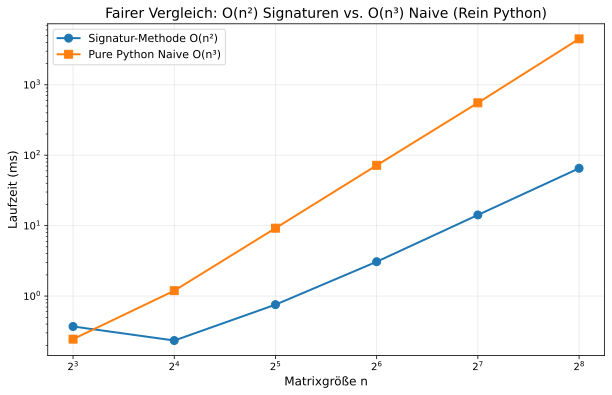
\includegraphics[width=0.85\textwidth]{experiment_boolean.pdf}
	\caption{Laufzeitvergleich Boolean Multiplikation ($O(n^2)$ vs. $O(n^3)$)}
	\label{fig:bmm}
\end{figure}

Die Ergebnisse zeigen, dass die Signatur-Methode bei einer Matrixgröße von $n=8$ noch einen geringfügigen Overhead aufweist. Ab $n=16$ kehrt sich dieses Verhältnis signifikant um. Bei $n=256$ erreicht die Signatur-Methode eine Laufzeit von ca. $65.24$ms, während die naive Multiplikation $4485.82$ms benötigt. Dies entspricht einem Speedup-Faktor von ca. $68,76$. Die quadratische Skalierung der Signatur-Methode gegenüber der kubischen Skalierung des naiven Ansatzes wird experimentell bestätigt.

\subsection{k-beschränkte Matrixmultiplikation}Im zweiten Experiment erfolgt der Vergleich des Schichten-Signatur-Verfahrens mit dem Strassen-Algorithmus für variierende Werte von $k$ und $n$. Während die Signatur-Methode eine theoretische Komplexität von $O(k \cdot n^2)$ aufweist, skaliert Strassen mit $O(n^{2,807})$.

\begin{figure}[htbp]
	\centering
	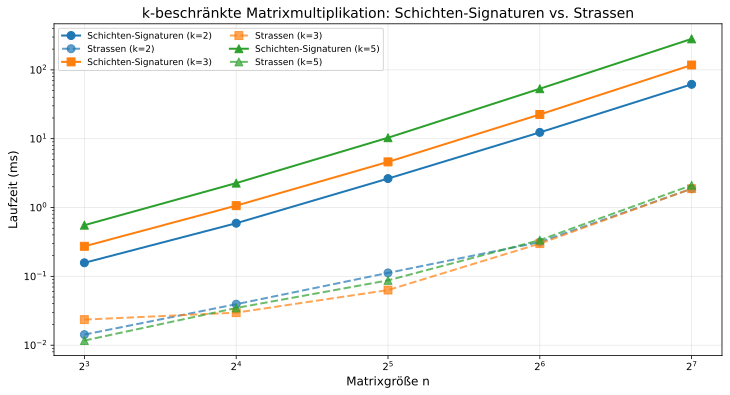
\includegraphics[width=0.85\textwidth]{experiment_k_bounded.pdf}
	\caption{Skalierung der Schichten-Signaturen bei variierendem $k$}
	\label{fig:k-bmm}
\end{figure}

Es zeigt sich, dass der Strassen-Algorithmus in der aktuellen Python-Umgebung bei kleinen Werten von $k$ effizienter arbeitet. Bei $n=128$ und $k=5$ benötigt die Schichten-Signatur $281.93$ms, während Strassen die Berechnung in $2.11$ms abschließt. Dies ist primär auf den hohen Rechenaufwand bei der Erzeugung sehr großer Signaturen (Bitbreite entspricht $n$) in Python zurückzuführen. Das Schichten-Verfahren weist jedoch die erwartete lineare Abhängigkeit von $k$ auf: Eine Erhöhung von $k=2$ auf $k=5$ resultiert in einer annähernd proportionalen Steigerung der Laufzeit.

\section{Zusammenfassung}

Die vorliegende Arbeit zeigt, dass die Signatur-Technik aus dem Subgraph-Algorithmus eine effiziente Alternative zur Berechnung der Boolean Matrixmultiplikation darstellt. Durch die Abbildung von Binärvektoren auf polynomiale Hash-Werte wird die logische Verknüpfung auf hardwarenahe Bitoperationen reduziert, was eine Reduktion der theoretischen Komplexität ermöglicht.

\subsection{Anwendungen}
Die Relevanz einer performanten Boolean Matrixmultiplikation in $O(n^2)$ erstreckt sich über verschiedene informatische Fachbereiche:
\begin{itemize}
	\item[-] \textbf{Graphentheorie:} Effiziente Berechnung der transitiven Hülle, Prüfung der Pfadexistenz sowie Lösung des All-Pairs Shortest Paths Problems durch wiederholte Anwendung der Multiplikation.
	\item[-] \textbf{Formale Verifikation:} Strukturelle Analyse von Abstract Syntax Trees (AST), Bestimmung der Ähnlichkeit von Programmen sowie Überprüfung von Zustandsüber\-gängen in Graphtransformationssystemen.
	\item[-] \textbf{Datenbanksysteme:} Optimierung relationaler Joins, Durchführung transitiver Abfragen in Graphdatenbanken sowie die Modellierung der Zugriffsrechte-Propagation in komplexen Netzwerken.
\end{itemize}

\subsection{Abschließende Betrachtung}
Durch die Anwendung der Signatur-Methode auf die Boolean Matrixmultiplikation lassen sich folgende Ergebnisse festhalten:
\begin{itemize}
	\item[-] Die theoretische Laufzeit von $O(n^2)$ stellt für diesen Spezialfall der Matrixmultiplikation das theoretische Optimum dar.
	\item[-] Die praktische Umsetzung profitiert unmittelbar von modernen CPU-Instruktionen für Bit-Arithmetik, wodurch der algorithmische Vorteil direkt in messbare Performancegewinne umgesetzt wird.
	\item[-] Der algebraische Korrektheitsbeweis bestätigt die verlustfreie Abbildung der logischen Operationen auf die Signatur-Ebene.
\end{itemize}

Die strukturelle Verwandtschaft zwischen dem Subgraph-Algorithmus und der vorgestellten Matrixmultiplikation unterstreicht die Vielseitigkeit der Signatur-Technik:

\begin{center}
	\begin{tabular}{|l|l|}
		\hline
		\textbf{Subgraph-Algorithmus} & \textbf{Boolean MatMul} \\
		\hline
		Spalten-Signaturen & Zeilen- und Spalten-Signaturen \\
		Zyklische Rotation & Bitweise UND-Operation \\
		LCS-Vergleich & OR-Check auf Bitebene (Ergebnis $\neq 0$) \\
		Subgraph-Erkennung & Nachweis der Pfadexistenz \\
		\hline
	\end{tabular}
\end{center}

Beide Verfahren nutzen die polynomiale Hash-Funktion zur hocheffizienten Strukturkodierung und erzielen dadurch signifikante Laufzeitvorteile gegenüber klassischen, kombinatorischen Ansätzen.

\subsection{Implementierung}
Die Referenz-Implementierung des Algorithmus sowie die zugehörige Testumgebung wurden unter Nutzung von Claude AI erstellt. Der vollständige Quelltext ist unter \url{https://github.com/hjstephan/bool-mm} verfügbar. Das Repository enthält zudem einen automatisiert generierten Code-Coverage-Report im HTML-Format zur Dokumentation der Testgüte und Verlässlichkeit der Implementierung.

\end{document}
